\documentclass{report}
\usepackage{titlesec}
\usepackage{float}
\usepackage{rotating}

\titleformat{\chapter}[block]{\LARGE \bfseries}{Chapter \arabic{chapter}}{1em}{}[]
\title{First Flight Test Project}
\author{Shun Li, Zhewen Xing, Linhan Qiao }
\date{\today}

\begin{document}
\maketitle
\tableofcontents

\chapter{Objects}
Through this flight test, the following performance should be examined.

\section{Communication:}

The communication test mainly consist of 2 aspects:
\begin{itemize}
    \item Communication between the Icrest 2.0 and DJI M300 (along with
        ZenMuse Camera.)

        Processing the image and detecting the forest fire and smoke require
        high computational resources, which may cause the deficiency of the
        command and states communication between the Icrest 2.0 and DJI M300.

    \item Communication between the Icrest 2.0 and the ground monitoring
        computer.

        There is no screen of the Icrest 2.0, thus a real-time states
        monitoring from the ground is critical to the security and convenience.

        As long as the Icrest 2.0 and Ground
        monitoring computer are in the same Local Area Network(LAN), the states
        and even the videos processed by the detecting algorithm could be easily
        accessed by using `WiFi` and `ssh` tool.

        But in the future, we should seek for more long-distance connecting
        method, like radio modem.


\end{itemize}


\section{Navigation}

\begin{itemize}
    \item Joystick Commands:

        In this test, the Navigation method is based on the dji osdk ros command 
        `Joystick commands`. The drone will simply fly along the zigzag flight
        path as shown in the following figure. The flight path is generated by
        the onboard computer, and send the command to the drone step by step.
        \begin{figure}[H]
            \centering
            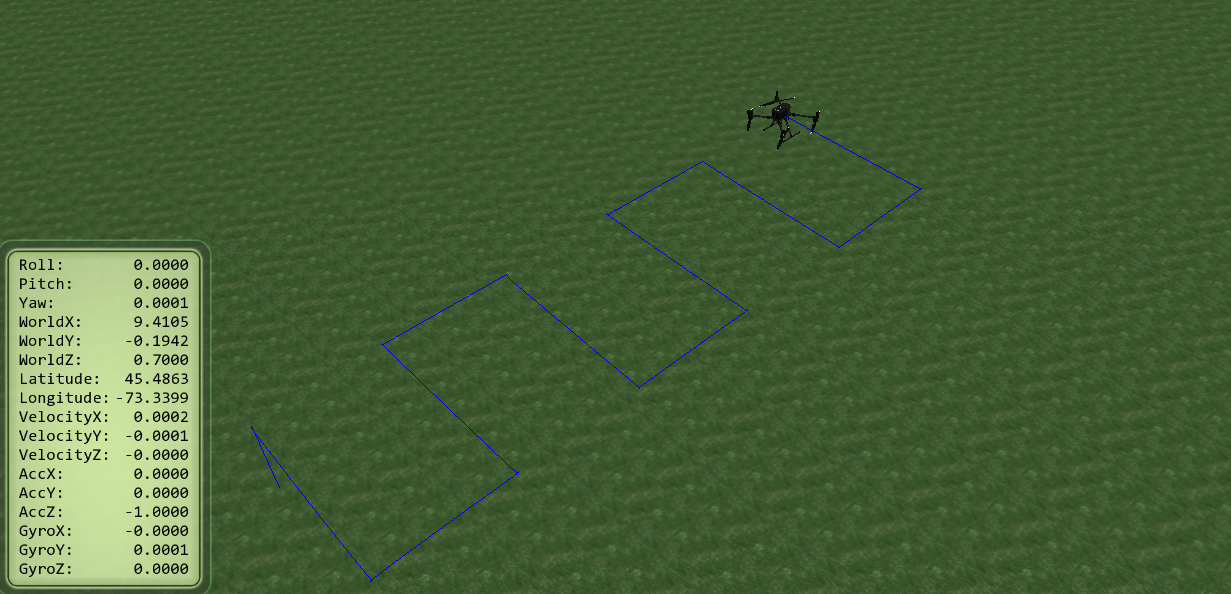
\includegraphics[width=1\textwidth]{./img/nav}
            \caption{the zigzag flight path}
        \end{figure}
\end{itemize}


\section{Fire and smoke detection:}
\begin{itemize}
    \item A Unet based forest fire and smoke segmentation algorithm will be
        tested on line with the ZenMuse camera. More specifically, the detecting
        speed and segmentation accuracy are tested. The indoor real time test is
        shown in the following figure:

    \item In this task, both original and masked video are stored as the database
        to be used in the future.
        \begin{figure}[H]
            \centering
            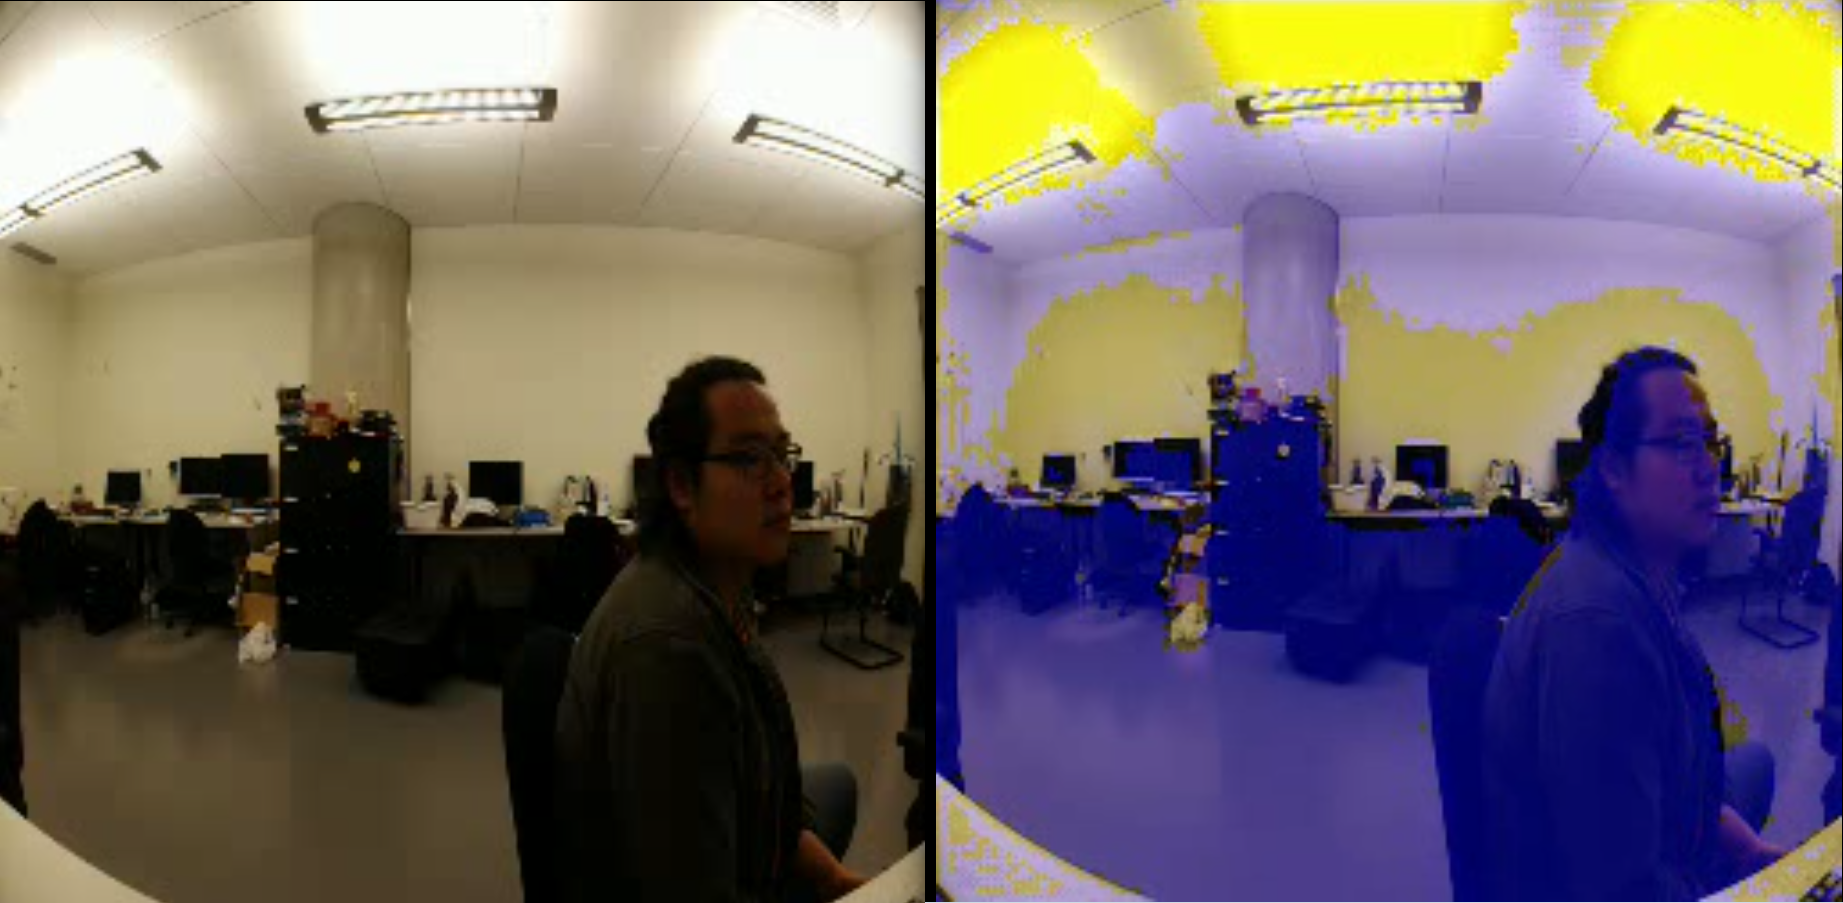
\includegraphics[width=0.8\textwidth]{./img/Screenshot from 2021-10-02 17-33-33.png}
            \caption{indoor test for fire and smoke detection}
        \end{figure}

\end{itemize}

Please note that we did not use the Infrared Image, because the deep learning
model is not ready to specify the thermal information.


\chapter{Schedule and Preparation}

\section{Date}
11, October 2021, which is Monday.

\section{Test Outline}
\begin{itemize}
    \item waypoint flight and detection
    \item data base image and video collection including the thermal and RGB
        imge from the ZenMuse camera.
\end{itemize}

\section{Preparation}
\begin{itemize}
    \item The portable power bank for the outdoor WiFi
    \item Oven and some woods to produce the fire and smoke.
\end{itemize}

\end{document}
